\subchapter{Bootloader - U-Boot}{Objectives: Set up serial
  communication, compile and install the U-Boot bootloader, use basic
  U-Boot commands, set up TFTP communication with the development
  workstation.}

As the bootloader is the first piece of software executed by a
hardware platform, the installation procedure of the bootloader is
very specific to the hardware platform. There are usually two cases:

\begin{itemize}

\item The processor offers nothing to ease the installation of the
  bootloader, in which case the JTAG has to be used to initialize
  flash storage and write the bootloader code to flash. Detailed
  knowledge of the hardware is of course required to perform these
  operations.

\item The processor offers a monitor, implemented in ROM, and through
  which access to the memories is made easier.

\end{itemize}

The Xplained board, which uses the SAMA5D3 SoCs, falls into the second
category. The monitor integrated in the ROM reads the MMC/SD card to
search for a valid bootloader before looking at the internal NAND
flash for a bootloader. In case nothing is available, it will operate
in a fallback mode, that will allow to use an external tool
to reflash some bootloader through USB. Therefore, either by using an MMC/SD
card or that fallback mode, we can start up a SAMA5D3-based board
without having anything installed on it.

\section{Downloading Microchip's flashing tool}

Go to the \code{~/embedded-linux-labs/bootloader} directory.

We're going to use that fallback mode, and its associated tool,
\code{sam-ba}.

We first need to download this tool, from Microchip's website\footnote{
In case this website is down, you can also find this
tool on \url{https://bootlin.com/labs/tools/}.}.

\begin{verbatim}
wget https://ww1.microchip.com/downloads/en/DeviceDoc/sam-ba_2.15.zip
unzip sam-ba_2.15.zip
\end{verbatim}

\section{Setting up serial communication with the board}

Plug the USB-to-serial cable on the Xplained board. The blue end of
the cable is going to \code{GND} on \code{J23}, red on \code{RXD} and
green on \code{TXD}. When plugged in your computer, a serial port
should appear, \code{/dev/ttyUSB0}.

\begin{center}
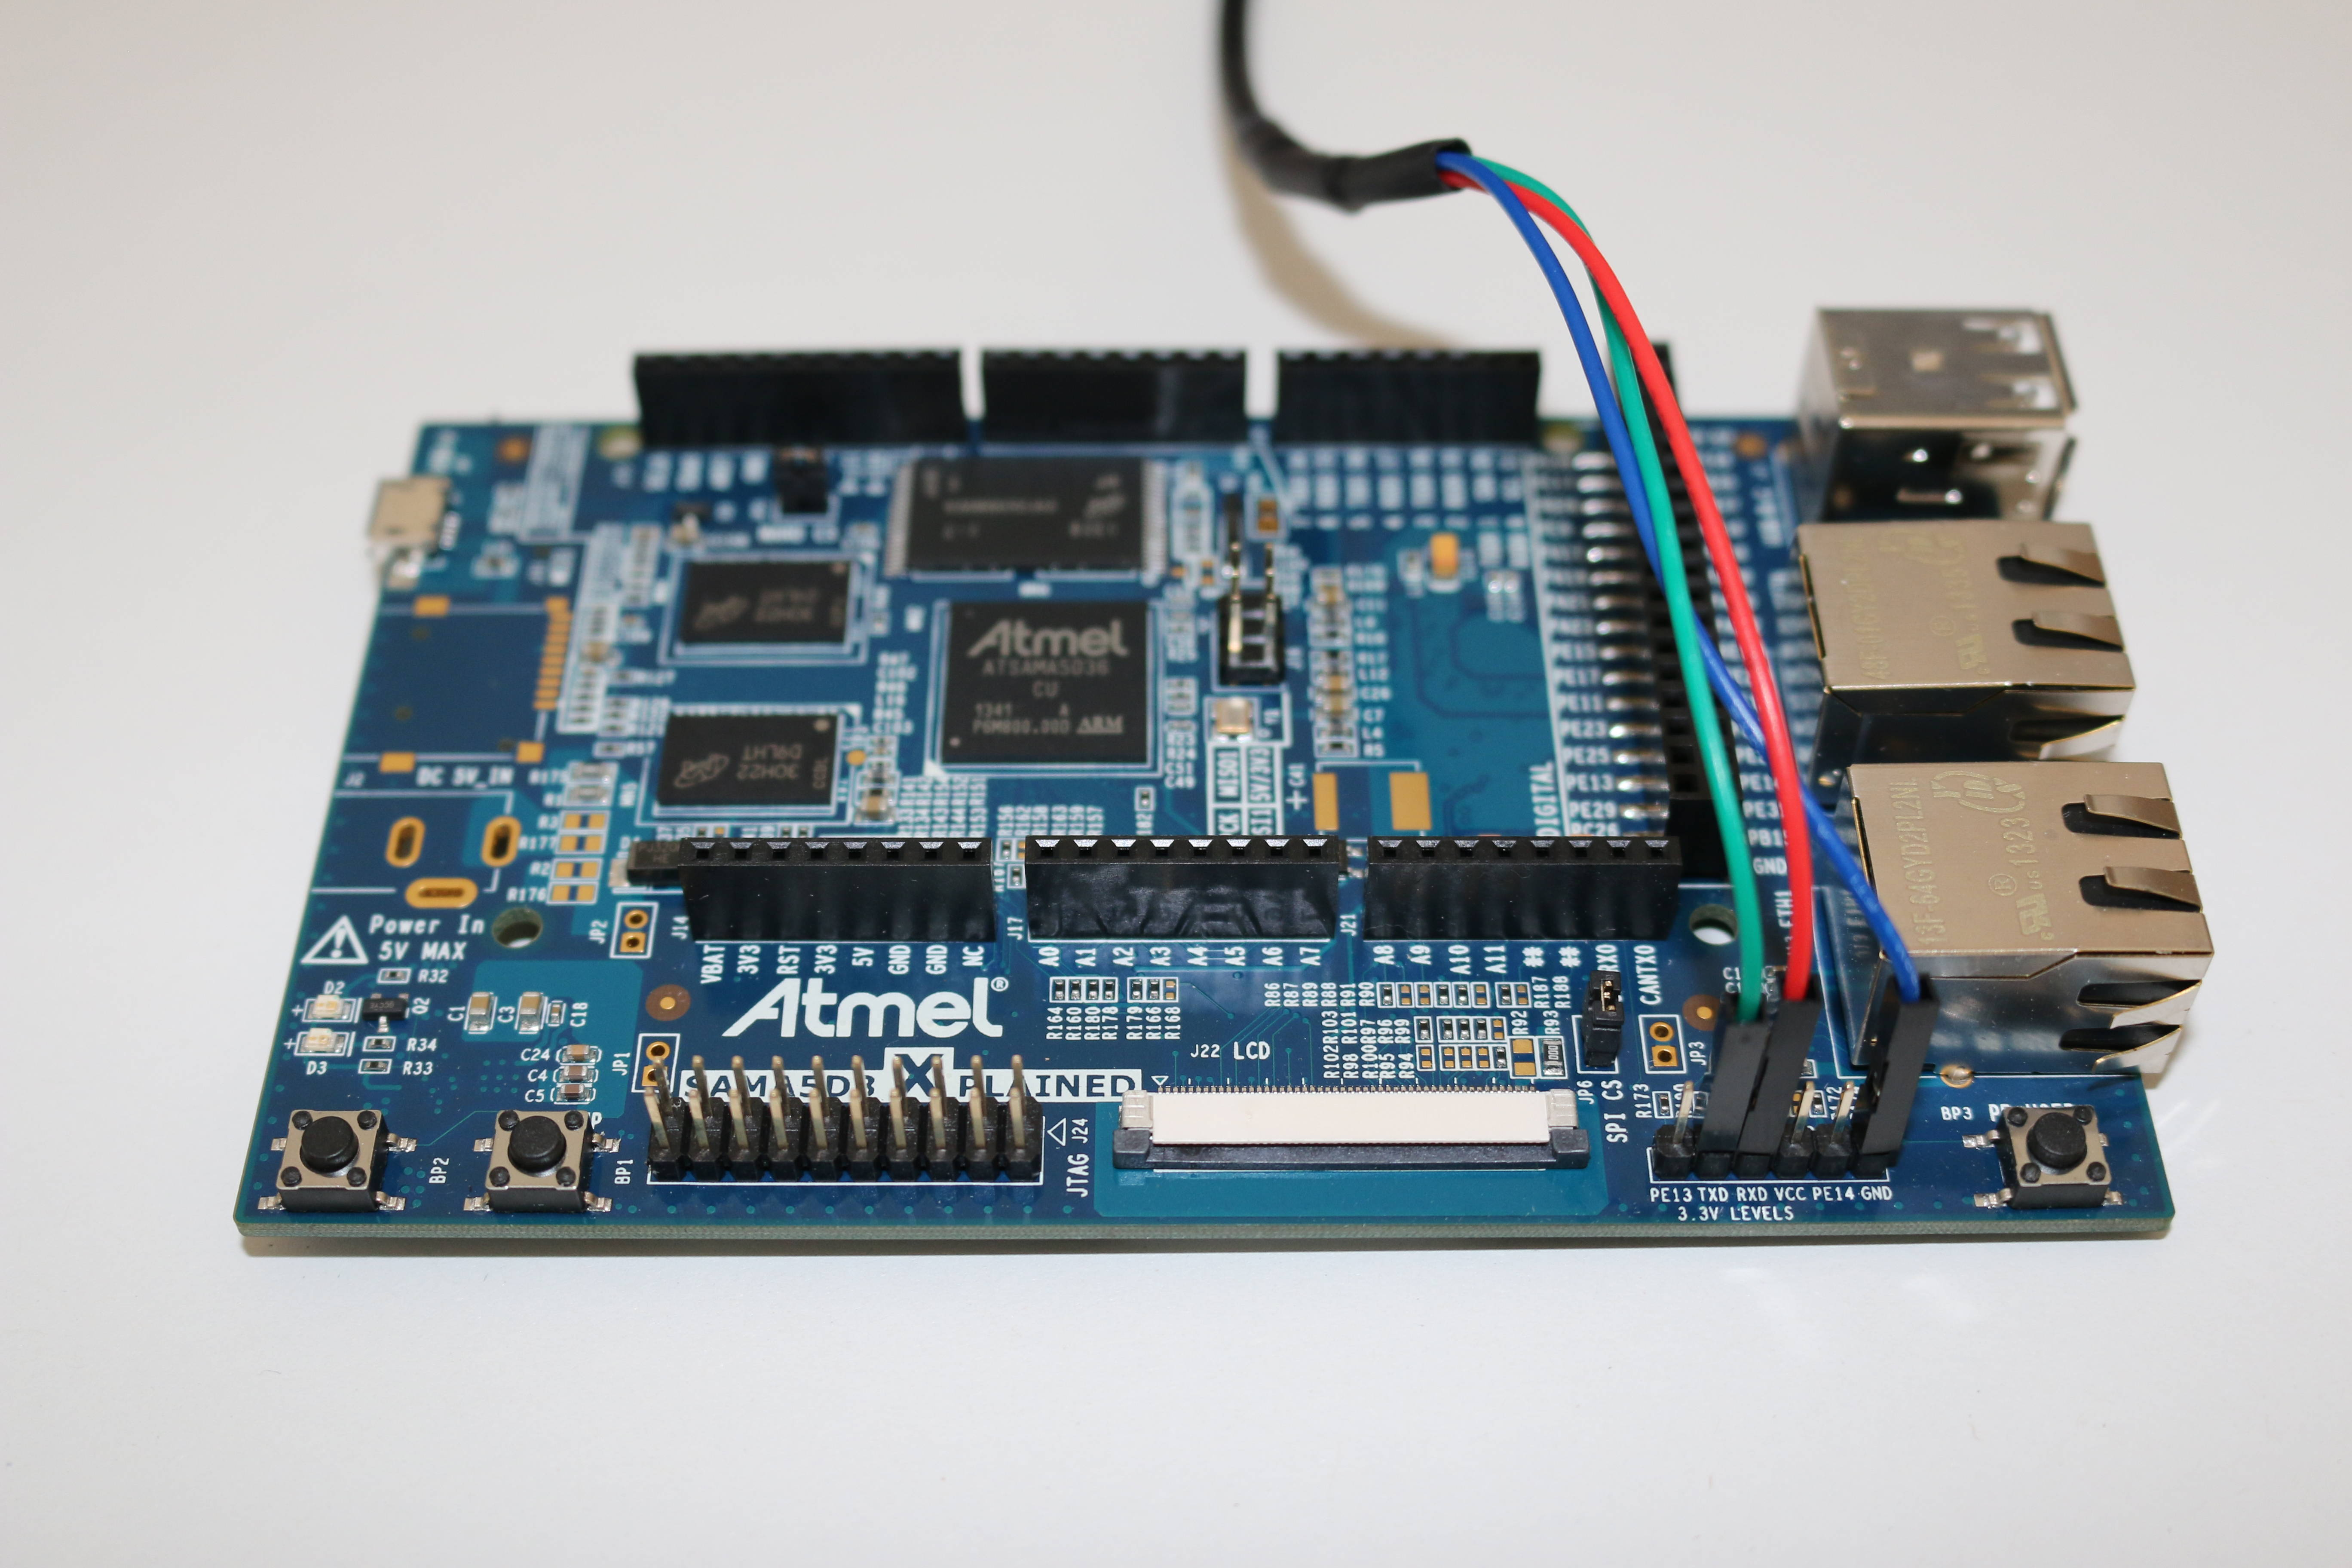
\includegraphics[width=8cm]{labs/sysdev-u-boot/xplained-serial-connector.jpg}
\end{center}

You can also see this device appear by looking at the output of
\code{dmesg}.

To communicate with the board through the serial port, install a
serial communication program, such as \code{picocom}:

\begin{verbatim}
sudo apt install picocom
\end{verbatim}

You also need to make your user belong to the \code{dialout} group to be
allowed to write to the serial console:

\begin{verbatim}
sudo adduser $USER dialout
\end{verbatim}

{\bf Important}: for the group change to be effective, in Ubuntu 18.04, you have to
{\em completely reboot} the system \footnote{As explained on
\url{https://askubuntu.com/questions/1045993/after-adding-a-group-logoutlogin-is-not-enough-in-18-04/}.}.
A workaround is to run \code{newgrp dialout}, but it is not global.
You have to run it in each terminal.

Run \code{picocom -b 115200 /dev/ttyUSB0}, to start serial
communication on \code{/dev/ttyUSB0}, with a baudrate of 115200.

You can now power-up the board by connecting the micro-USB cable to 
the board, and to your PC at the other end. If a system was previously
installed on the board, you should be able to interact with it
through the serial line.

If you wish to exit \code{picocom}, press \code{[Ctrl][a]} followed by
\code{[Ctrl][x]}.

\section{AT91Bootstrap Setup}

The boot process is done in two steps with the ROM monitor trying to
execute a first piece of software, called \em{AT91Bootstrap}, from
its internal SRAM, that will initialize the DRAM, load \em{U-Boot}
that will in turn load Linux and execute it.

As far as bootloaders are concerned, the layout of the NAND flash will
look like:

\begin{center}
  \includegraphics[width=\textwidth]{labs/sysdev-u-boot/flash-map.pdf}
\end{center}

\begin{itemize}
\item Offset \code{0x0} for the first stage bootloader is dictated by
  the hardware: the ROM code of the SAMA5D3 looks for a bootloader at
  offset \code{0x0} in the NAND flash.
\item Offset \code{0x40000} for the second stage bootloader is decided
  by the first stage bootloader. This can be changed by changing the
  AT91Bootstrap configuration.
\item Offset \code{0xc0000} of the U-Boot environment is decided by
  U-Boot. This can be changed by modifying the U-Boot configuration.
\end{itemize}

The first item to compile is AT91Bootstrap that you can fetch from
Microchip's GitHub account:

\begin{verbatim}
git clone https://github.com/linux4sam/at91bootstrap.git
cd at91bootstrap
git checkout v3.8.9
\end{verbatim}

Then, we first need to configure the build system for our setup. We're
going to need a few pieces of information for this:

\begin{itemize}
\item Which board you want to run AT91Bootstrap on
\item Which device should AT91Bootstrap will be stored on
\item What component you want AT91Boostrap to load
\end{itemize}

You can get the list of the supported boards by listing the
\code{board} directory. You'll see that in each of these folders, we
have a bunch of \code{defconfig} files, that are the supported
combinations. In our case, using the Atmel SAMA5D3 Xplained
board, we will load U-Boot, from NAND flash on
(\code{nf} in the \code{defconfig} file names).

After finding the right \code{defconfig} file, load it using
\code{make <defconfig_filename>} (just the file name, without
the directory part).

In recent versions of AT91Bootstrap, you can now run \code{make
menuconfig} to explore options available in this program. 

The next thing to do is to specify the cross-compiler prefix
(the part before \code{gcc} in the cross-compiler executable name):

\begin{verbatim}
export CROSS_COMPILE=arm-linux-
\end{verbatim}

Last but not least, install the \code{python} package
that the Makefile for AT91Bootstrap will try to invoke.

You can now start compiling using \code{make}\footnote{You can
speed up the compiling by using the \code{-jX} option with
\code{make}, where X is the number of parallel jobs used for
compiling. Twice the number of CPU cores is a good value.}.

At the end of the compilation, you should have a file called
\code{sama5d3_xplained-nandflashboot-uboot-*.bin}, in the
\code{binaries} folder.

In order to flash it, we need to do a few things. First, remove the
\code{NAND CS} jumper on the board. It's next to the pin header
closest to the Micro-USB plug. Now, press the \code{RESET} button.
On the serial port, you should see \code{RomBoot}.

Put the jumper back.

Then, start \code{sam-ba_64}, running the executable from where
it was extracted. You'll get a small window. Select the \code{ttyACM0}
connection, and the \code{at91sama5d3x-xplained} board. Hit
\code{Connect}.

You need to:
\begin{itemize}
\item Hit the \code{NANDFlash} tab
\item In the \code{Scripts} choices, select \code{Enable NandFlash}
      and hit \code{Execute}
\item Select \code{Erase All}, and execute the command
\item Then, select and execute \code{Enable OS PMECC parameters}
  in order to change the NAND ECC parameters to what RomBOOT expects.
\item Finally, send the image we just compiled using the command
  \code{Send Boot File}
\end{itemize}

AT91Bootstrap should be flashed now, keep \code{sam-ba} open, and move to
the next section.

\section{U-Boot setup}

Download U-Boot:

\begin{verbatim}
wget ftp://ftp.denx.de/pub/u-boot/u-boot-2017.09.tar.bz2
\end{verbatim}

More recent versions may also work, but we have not tested them.

Extract the source archive and get an understanding of U-Boot's
configuration and compilation steps by reading the \code{README} file,
and specifically the {\em Building the Software} section.

Basically, you need to:

\begin{itemize}

\item Set the \code{CROSS_COMPILE} environment variable;

\item Run \code{make <NAME>_defconfig}, where the list of available
  configurations can be found in the \code{configs/} directory. There
  are two flavors of the Xplained configuration: one to run from the
  SD card (\code{sama5d3_xplained_mmc}) and one to run from the NAND
  flash (\code{sama5d3_xplained_nandflash}). Since we're going to boot
  on the NAND, use the latter.

\item Now that you have a valid initial configuration, you can now
  run \code{make menuconfig} to further edit your bootloader features. 

\item In recent versions of U-Boot and for some boards, you will
  need to have the Device Tree compiler:

\begin{verbatim}
sudo apt install device-tree-compiler
\end{verbatim}

\item Finally, run \code{make}, which should build U-Boot.

\end{itemize}

\section{Shrinking U-Boot}

Look at the size of the \code{u-boot.bin} binary. According to the above
flash layout, the U-Boot binary is supposed to fit between flash offset
\code{0x40000} and offset \code{0xc0000}, corresponding to a maximum
size of \code{524288} bytes. Is \code{u-boot.bin} bigger than this
maximum?

The first offset is what AT91Bootstrap expects
(though it can be changed in AT91Bootstrap's configuration.
The second one, corresponding to where U-Boot stores its environment
settings, is board dependent but apparently cannot be changed
through \code{make menuconfig}. 

To avoid recompiling AT91Bootstrap, we propose to compile U-Boot with
less features, to make its binary small. That's probably something you
will do too during real-life projects.

So, in U-Boot sources, run \code{make menuconfig}, look for and disable
the below options:\footnote{For each option, don't hesitate to use
help information to find out what it is about}.

\begin{itemize}
\item \code{ext4} options
\item \code{nfs} options
\item \code{USB} options
\item \code{SPL} options
\item \code{XIMG} support
\item \code{FIT} (Flattened Image Tree) support
\item \code{CMD_ELF} option
\item \code{dhcp} command support
\item Regular expression support (\code{REGEX})
\item \code{loadb} support
\item \code{CMD_MII} option
\end{itemize}

Now, recompile U-Boot and check that \code{u-boot.bin} is smaller
than our maximum size.

\section{Flashing U-Boot}

Now, in \code{sam-ba}, in the \code{Send File Name} field, set the path to
the \code{u-boot.bin} that was just compiled, and set the address to
\code{0x40000}. Click on the \code{Send File} button.

You can now exit \code{sam-ba}.

\section{Testing U-Boot}

Reset the board and check that it boots your new bootloaders. You can
verify this by checking the build dates:

\begin{verbatim}
AT91Bootstrap 3.9.1 (Sun May  3 08:10:48 CEST 2020)

NAND: ONFI flash detected
NAND: Manufacturer ID: 0x2c Chip ID: 0xda
NAND: Page Bytes: 2048, Spare Bytes: 64
NAND: ECC Correctability Bits: 4, ECC Sector Bytes: 512
NAND: Disable On-Die ECC
NAND: Initialize PMECC params, cap: 4, sector: 512
NAND: Image: Copy 0xc0000 bytes from 0x40000 to 0x26f00000
NAND: Done to load image
<debug_uart> 

U-Boot 2020.04 (May 03 2020 - 08:47:45 +0200)

CPU: SAMA5D36
Crystal frequency:       12 MHz
CPU clock        :      528 MHz
Master clock     :      132 MHz
DRAM:  256 MiB
NAND:  256 MiB
MMC:   Atmel mci: 0, Atmel mci: 1
Loading Environment from NAND... *** Warning - bad CRC, using default environment

In:    serial@ffffee00
Out:   serial@ffffee00
Err:   serial@ffffee00
Net:   
Error: ethernet@f0028000 address not set.

Error: ethernet@f802c000 address not set.
No ethernet found.

Hit any key to stop autoboot:  0 
\end{verbatim}


Interrupt the countdown to enter the U-Boot shell:
\begin{verbatim}
=>
\end{verbatim}

In U-Boot, type the \code{help} command, and explore the few commands
available.

\section{Setting up Ethernet communication}

Later on, we will transfer files from the development workstation to
the board using the TFTP protocol, which works on top of an Ethernet
connection.

To start with, install and configure a TFTP server on your development
workstation, as detailed in the bootloader slides.

With a network cable, connect the Ethernet port labelled ETH0/GETH of
your board to the one of your computer. If your computer already has a
wired connection to the network, your instructor will provide you with
a USB Ethernet adapter. A new network interface should appear on your
Linux system.

Find the name of this interface by typing:
\begin{verbatim}
ifconfig -a
\end{verbatim}

The network interface name is likely to be
\code{enxxx}\footnote{Following the {\em Predictable Network Interface
Names} convention:
\url{https://www.freedesktop.org/wiki/Software/systemd/PredictableNetworkInterfaceNames/}}.
If you have a pluggable Ethernet device, it's easy to identify as it's
the one that shows up after pluging in the device.

Then, instead of configuring the host IP address from NetWork Manager’s graphical interface,
let’s do it through its command line interface, which is so much easier to use:

\begin{verbatim}
nmcli con add type ethernet ifname en... ip4 192.168.0.1/24
\end{verbatim}

Now, configure the network on the board in U-Boot by setting the \code{ipaddr}
and \code{serverip} environment variables:

\begin{verbatim}
setenv ipaddr 192.168.0.100
setenv serverip 192.168.0.1
\end{verbatim}

The first time you use your board, you also need to set the MAC
address in U-boot:

\begin{verbatim}
setenv ethaddr 12:34:56:ab:cd:ef
\end{verbatim}

In case the board was previously configured in a different way, we
also turn off automatic booting after commands that can be used to
copy a kernel to RAM:

\begin{verbatim}
setenv autostart no
\end{verbatim}

To make these settings permanent, save the environment:

\begin{verbatim}
saveenv
\end{verbatim}

Now reset your board\footnote{Resetting your board is needed to
make your \code{ethaddr} permanent, for obscure reasons. If you
don't, U-boot will complain that \code{ethaddr} is not
set.}.

You can then test the TFTP connection. First, put a small text file in
the directory exported through TFTP on your development
workstation. Then, from U-Boot, do:

\begin{verbatim}
tftp 0x22000000 textfile.txt
\end{verbatim}

The \code{tftp} command should have downloaded the
\code{textfile.txt} file from your development workstation into
the board's memory at location \code{0x22000000}\footnote{
This location is part of the board DRAM. If you want
to check where this value comes from, you can check the Atmel SAMA5D3
datasheet at \url{https://bit.ly/2GTZYVs}. It's a big document (more than 1,800
pages). In this document, look for \code{Memory Mapping} and you
will find the SoC memory map. You will see that the address range for
the memory controller ({\em DDRC S}) starts at \code{0x20000000}
and ends at \code{0x3fffffff}. This shows that the \code{0x22000000} 
address is within the address range for RAM. You can also try with other
values in the same address range, knowing that our board only has 256 MB
of RAM (that's \code{0x10000000}, so the physical RAM probably ends at
\code{0x30000000}).}.

You can verify that the download was successful by dumping the
contents of the memory:

\begin{verbatim}
md 0x22000000
\end{verbatim}

We will see in the next labs how to use U-Boot to download, flash and
boot a kernel.

\section{Rescue binaries}

If you have trouble generating binaries that work properly, or later
make a mistake that causes you to loose your bootloader binaries, you
will find working versions under \code{data/} in the current lab
directory.
